\documentclass[../report.tex]{subfiles}


\begin{document}
% --------------------------------------------------------------------------
% SECTION 4 
% --------------------------------------------------------------------------
\section{HIL}

\textbf{System name:} One wheel skateboard\\
\textbf{List of files:} 
\begin{tabular}{ |c|c| }
    \hline
    main.m & Parameters initialization \\
    model.slx & Main model \\
    dataOneWheel.mat & Data from accelerometer from mobile Matlab app\\
    \hline
\end{tabular} \\
\textbf{Datasheets:}
\begin{tabular}{ |c|c| }
    \hline
    adxl335.pdf & Accelerometer \\
    lts\_6-np.pdf & LEM sensor \\
    moc23series.pdf & DC motor \\
    \hline
\end{tabular} \\

\subsection{Selection and description of the controlled system}
Modeled system is one wheel skateboard \ref{fig:one_wheel}. 

\begin{figure}[htb!]
    \centering
    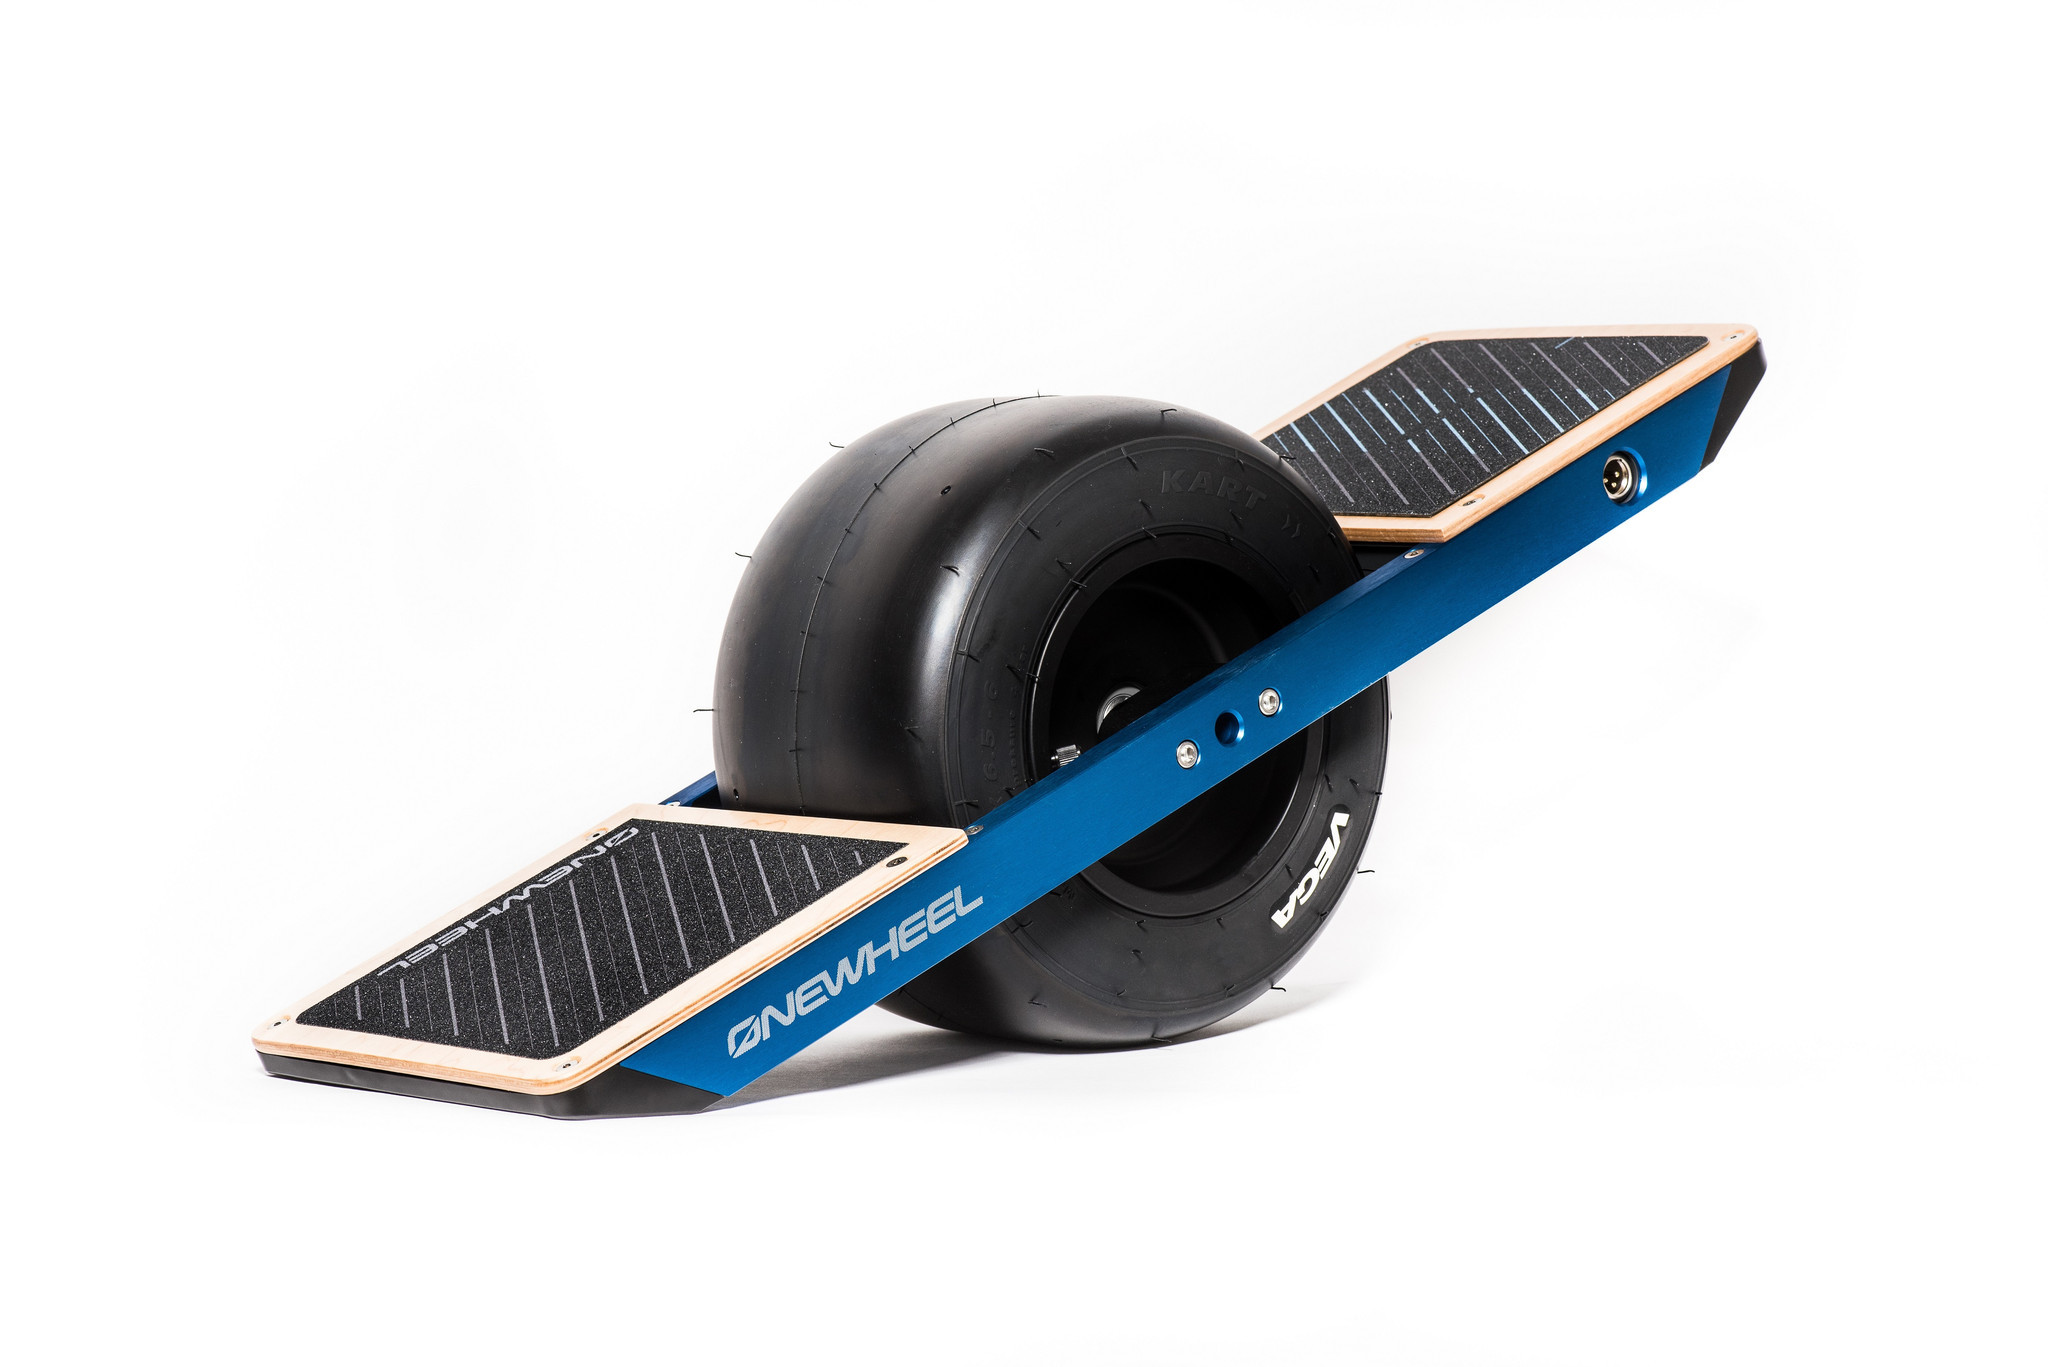
\includegraphics[width=0.8\textwidth]{one_wheel.jpeg}
    \caption{One Wheel \cite{one_wheel}}
    \label{fig:one_wheel}
\end{figure}

The simplify model of the one wheel skateboard system features a DC motor,
accelerometer and control unit \ref{fig:one_wheel_simp}.

\begin{figure}[htb!]
    \centering
    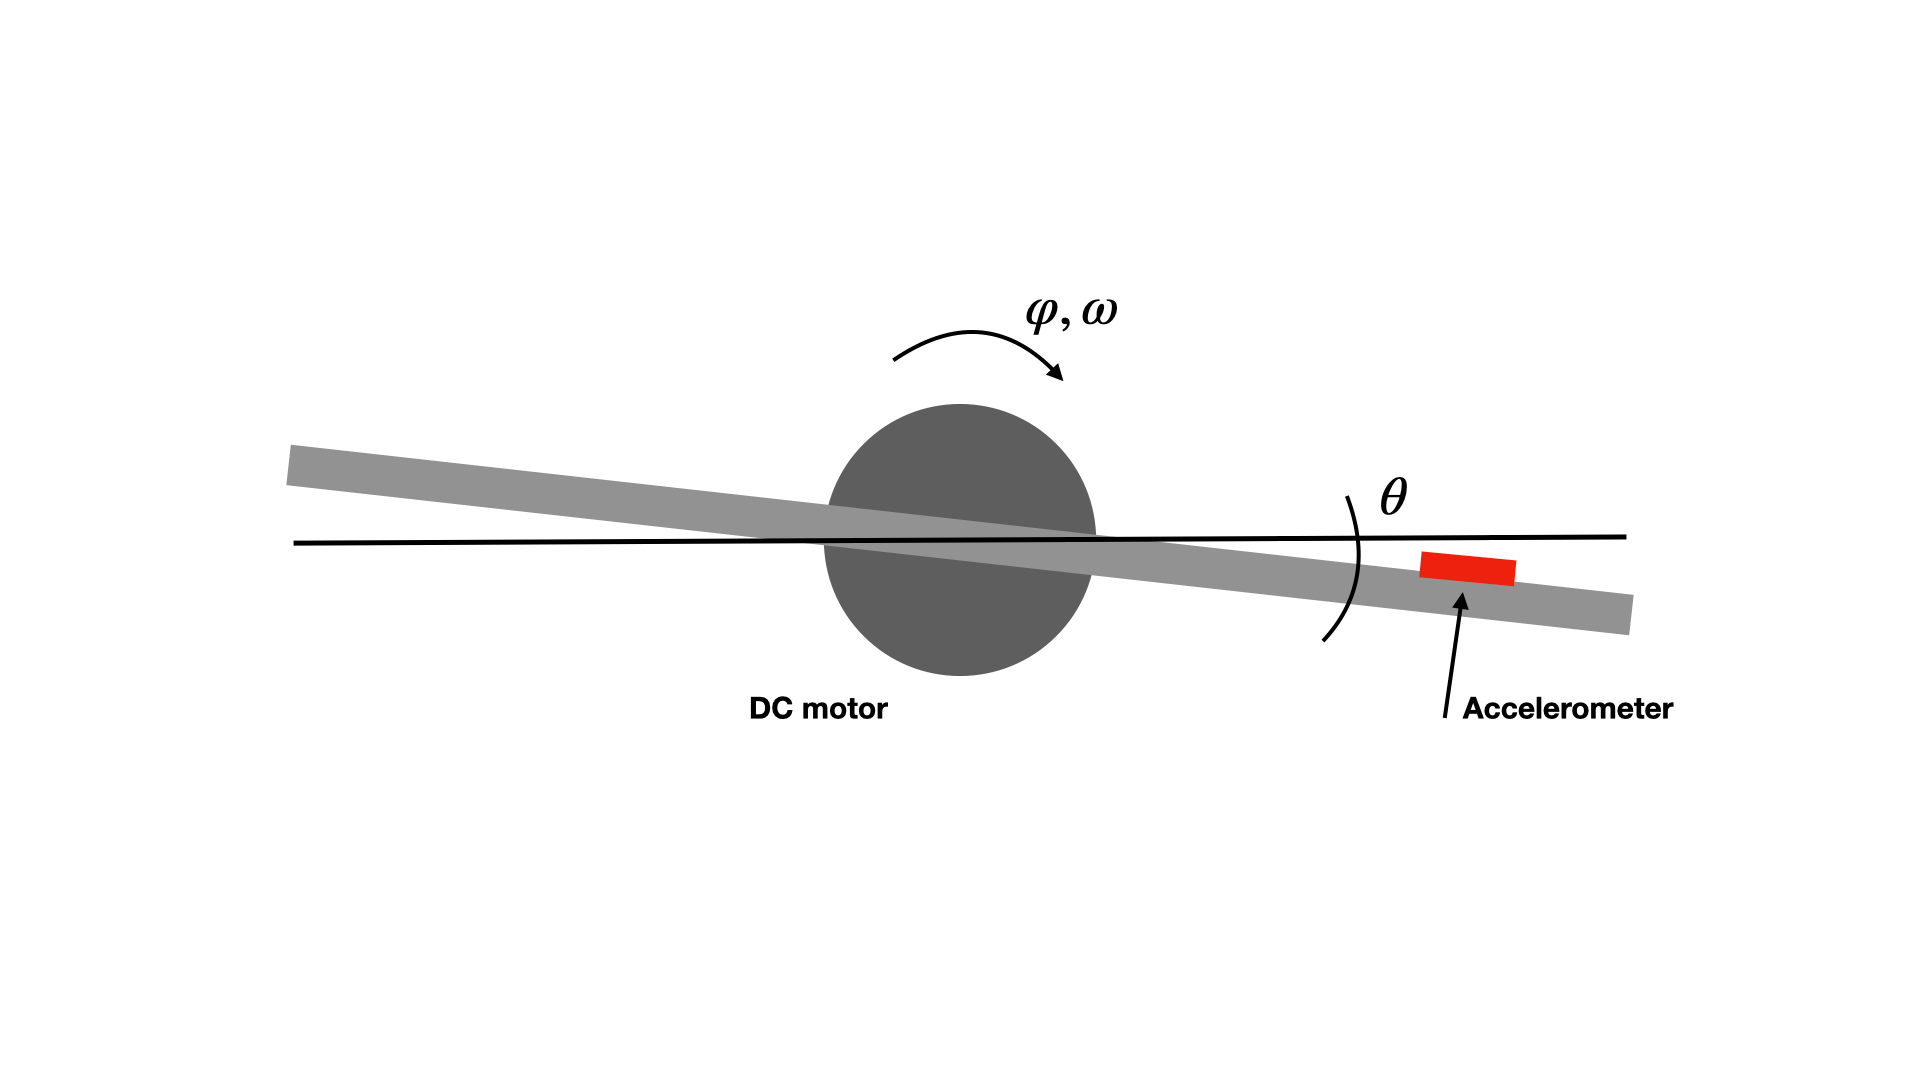
\includegraphics[width=0.8\textwidth]{one_wheel_simp.png}
    \caption{One Wheel simplify model}
    \label{fig:one_wheel_simp}
\end{figure}

\subsection{Model of a controlled system in Simulink}
Controlled system is DC motor with digital controlled H-bridge
\ref{fig:controlled_system}
\begin{figure}[htb!]
    \centering
    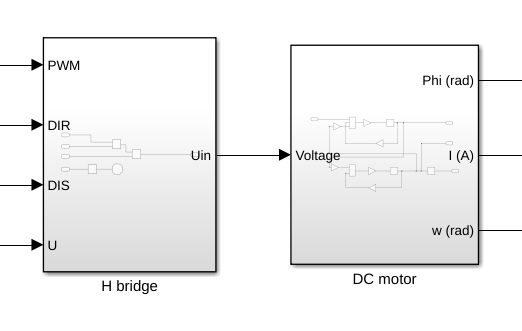
\includegraphics[width=0.6\textwidth]{controlled_system.png}
\caption{Controlled system Simulink model}
    \label{fig:controlled_system}
\end{figure}

\subsection{Models of sensors and actuators}
As a sensors were used encoder with 2 channels A and B to measure position
and velocity of dc motor. LEM sensor to measure current in dc motor
\ref{fig:sensors1}. And accelerometer sensor that provide accelerations in
3-axis. Accelerations recalculated to angle (pitch) for stabilizing a
system and provide acceleration from dc motor \ref{fig:sensors2}.
\begin{figure}[hbt!]
    \centering
    \begin{minipage}{.5\textwidth}
    \centering
    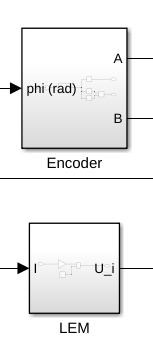
\includegraphics[width=0.3\textwidth]{sensors1.png}
    \caption{Encoder and LEM sensors}
    \label{fig:sensors1}
\end{minipage}%
\begin{minipage}{.5\textwidth}
    \centering
    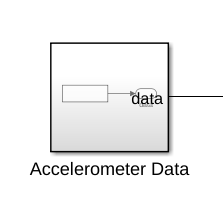
\includegraphics[width=0.4\textwidth]{sensors2.png}
    \caption{Accelerometer sensor}
    \label{fig:sensors2}
\end{minipage}
\end{figure}

\subsection{Control unit and signal adaptation}
Control Unit process acceleration data, LEM sensor data and motor actual
velocity \ref{fig:control_unit1}.

\begin{figure}[hbt!]
    \centering
    \begin{minipage}{.5\textwidth}
    \centering
    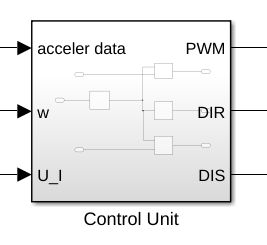
\includegraphics[width=0.5\textwidth]{controll_unit_1.png}
\caption{Control sub-block}
\label{fig:control_unit1}
\end{minipage}%
\begin{minipage}{.5\textwidth}
    \centering
    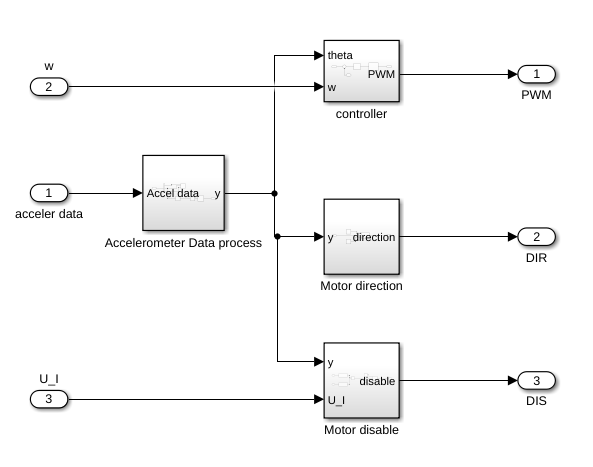
\includegraphics[width=1\textwidth]{controll_unit2.png}
    \caption{Control unit}
    \label{fig:control_unit2}
\end{minipage}
\end{figure}

\subsection{Tests}

\subsubsection{Correct setup}
Correct setup with acceleration data from mobile Matlab application
\ref{fig:correct}.

\begin{figure}[htb!]
    \centering
    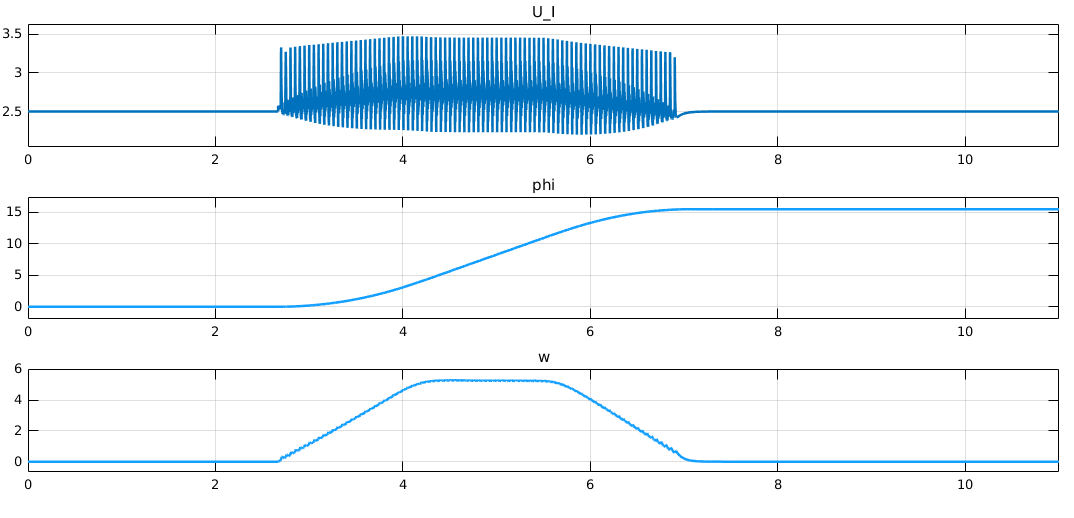
\includegraphics[width=0.8\textwidth]{correct_plot.png}
\caption{Correct setup test}
    \label{fig:correct}
\end{figure}
\subsubsection{Changing parameters}
Change rotor inertia from $J = 2189\cdot10^{-6} [kg/m^2]$ to $J = 1
[kg/m^2]$. Result is present in \ref{fig:change} graph.
\begin{figure}[htb!]
    \centering
    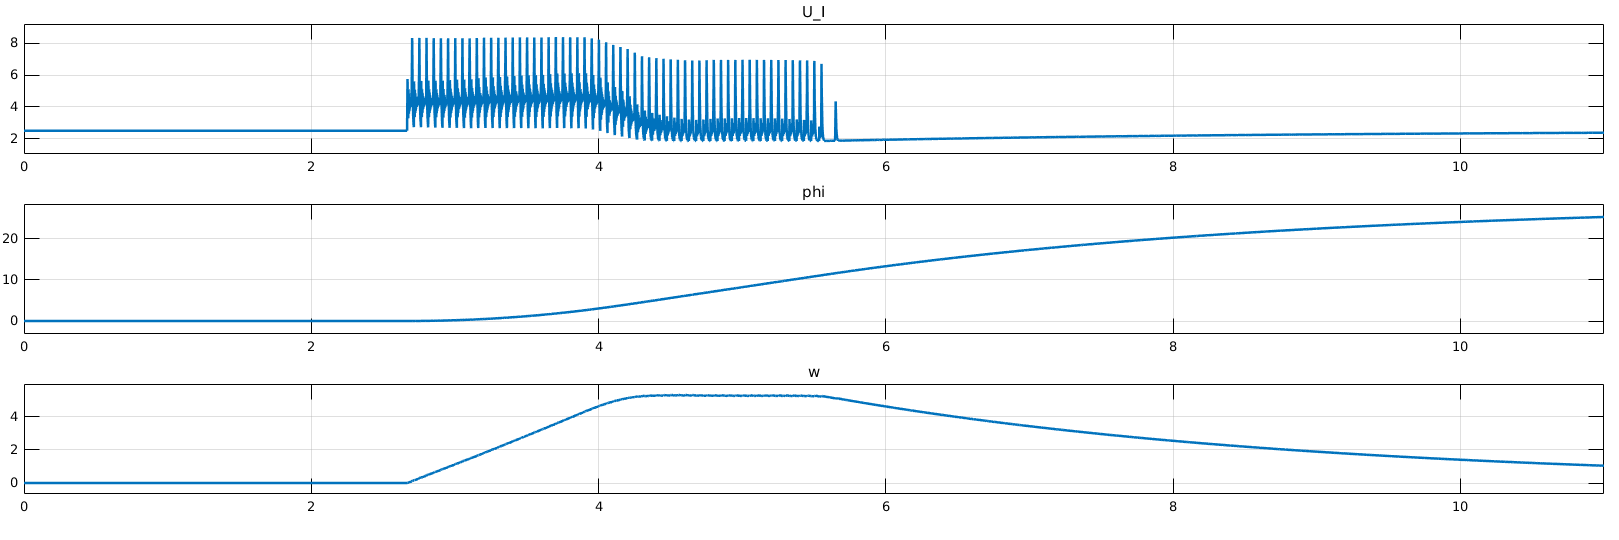
\includegraphics[width=0.8\textwidth]{change_params_plot.png}
\caption{Changing parameters test}
    \label{fig:change}
\end{figure}
\subsubsection{Fault setup}
Change the maximum pitch angle from $\varphi_max = 10 [rad]$ to $\varphi_max = 3
[rad]$ \ref{fig:fault}.
\begin{figure}[htb!]
    \centering
    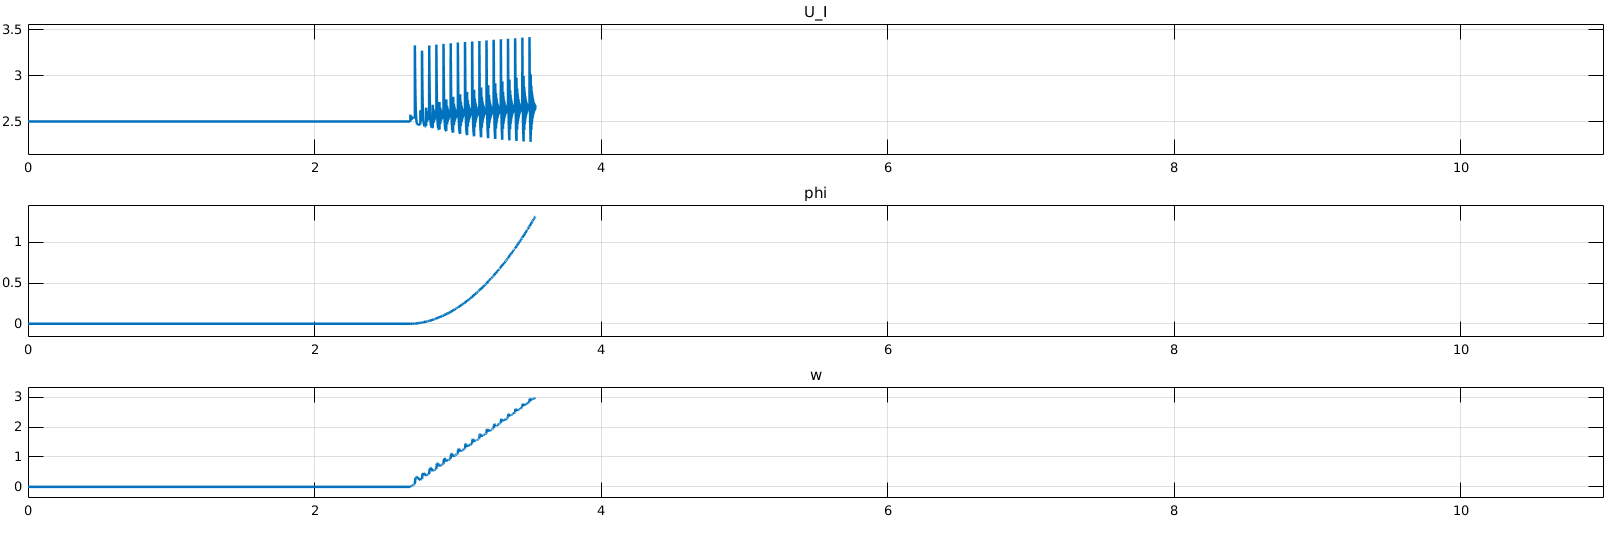
\includegraphics[width=0.8\textwidth]{fault_plot.png}
\caption{Fault setup test}
    \label{fig:fault}
\end{figure}
\subsection{Evaluation of the whole task and conclusion}
To control a real one wheel, it is necessary to use a gyroscope together
with an accelerometer.
The accuracy of the encoder model was insufficient to control the model, so
an analog signal was used.
Datasheet of used actuator and sensor are included.
\end{document}
